\documentclass[preprint]{sigplanconf}

\usepackage{amsmath}
\usepackage{amssymb}
\usepackage{alltt}
\usepackage{url}
\usepackage{natbib}
\usepackage{datetime}
\usepackage{graphicx}
\usepackage{comment}

%include polycode.fmt
%include play.fmt

% from the ICFP website
\bibpunct();A{},
\let\cite=\citep

% general stuff
\newcommand{\T}[1]{\texttt{#1}}
\newcommand{\C}[1]{\textsf{#1}}
\newcommand{\tup}[1]{\ensuremath{\langle #1 \rangle}}
\newcommand{\mtxt}[1]{\textsf{#1}}

\newcommand{\pic}[1]{\includegraphics[scale=0.55]{#1.eps}}

% examples
\newcounter{exmp}
\setcounter{exmp}{1}
\newcommand{\yesexample}{\subsubsection*{Example \arabic{exmp}}\refstepcounter{exmp}}
\newcommand{\noexample}{\hfill$\Box$}

\newcommand{\todo}[1]{\textbf{\textsc{Todo:} #1}}

% code blocks
\newenvironment{code}{\begin{alltt}\small}{\end{alltt}}
\newenvironment{codepage}
    {\begin{minipage}[h]{\textwidth}\begin{code}}
    {\end{code}\end{minipage}}

\newenvironment{example}{\yesexample}{\noexample}
\newenvironment{revisit}[1]{\subsubsection*{Example #1 (revisited)}}{\noexample}
\newenvironment{examplename}[1]
    {\subsubsection*{Example \arabic{exmp} (#1)}\refstepcounter{exmp}}
    {\noexample}

\newcommand{\K}{\ensuremath{^\ast}} % kleene star
\newcommand{\D}{\ensuremath{\cdot}} % central dot

\renewcommand{\c}[3]{\tup{\T{#1},\T{#2},\T{\{#3\}}}}
\newcommand{\cc}[2]{\c{#1}{$\lambda$}{#2}}

\newcommand{\s}[1]{\ensuremath{_{\tt #1}}} % subscript, in tt font
\newcommand{\g}[1]{\{#1\}} % group, put { } round it
\newcommand{\U}{\textunderscore}
\newcommand{\vecto}[1]{\overrightarrow{#1\;}}
\newcommand{\gap}{\;\;}
\newcommand{\dom}{\text{dom}}

\newcommand{\derive}{\textsc{Derive}}
\newcommand{\ignore}{}

\newcommand{\compare}[2]{\subsubsection*{\textsf{#1} from #2:}\vspace{-1ex}}


\begin{document}

\conferenceinfo{Haskell Workshop '07}{date, City.} %
\copyrightyear{2007} %
\copyrightdata{[to be supplied]}

\titlebanner{\today{} - \currenttime{}}        % These are ignored unless
\preprintfooter{}   % 'preprint' option specified.

\title{Uniform Boilerplate and List Processing}
\subtitle{\textit{Or}: Scrap Your Scary Types}

\authorinfo{Neil Mitchell}
           {University of York, UK}
           {\url{http://www.cs.york.ac.uk/~ndm/}}
\authorinfo{Colin Runciman}
           {University of York, UK}
           {\url{http://www.cs.york.ac.uk/~colin/}}

\maketitle

\begin{comment}
% extra code needed for tex2hs
\begin{code}
class Uniplate x where
	uniplate :: x -> ([x], [x] -> x)
\end{code}
\begin{code}
class Uniplate x where
\end{code}
\begin{code}
transform' x = transform x
\end{code}
\begin{code}
children_ = undefined
context = undefined
\end{code}
\end{comment}


\begin{abstract}
Generic traversals over recursive data structures are often referred to as \textit{boilerplate} code. The definitions of functions involving such traversals may repeat very similar patterns, but with variations for different data types and different functionality. This paper focuses on traversals where only one type has value-specific behaviour, requiring fewer type extensions than other boilerplate removal systems. The |Uniplate| class is introduced, which shows how all traversals can implemented in terms of a single operation.
\end{abstract}

\section{Introduction}

Take a simple example of a recursive data type:

\begin{code}
data Expr  =  Val  Int
           |  Var  String
           |  Neg  Expr
           |  Add  Expr  Expr
           |  Sub  Expr  Expr
           |  Mul  Expr  Expr
           |  Div  Expr  Expr
\end{code}

The |Expr| type represents a small expression language for integer expressions, which permits free variables.

\begin{example}
\label{ex:variables}

Suppose we need to extract a list of all the variables in an expression:

\begin{code}
variables :: Expr -> [String]
variables (Var  x    ) = [x]
variables (Val  x    ) = []
variables (Neg  x    ) = variables x
variables (Add  x y  ) = variables x ++ variables y
variables (Sub  x y  ) = variables x ++ variables y
variables (Mul  x y  ) = variables x ++ variables y
variables (Div  x y  ) = variables x ++ variables y
\end{code}

This definition has the following undesirable characteristics:

\begin{itemize}
\item adding a new constructor would require an additional equation;
\item the |++| operation is specified many times;
\item the code is highly repetitive and unnecessarily long;
\item the code cannot be shared with other similar operations.
\end{itemize}

This problem is referred to as the \textit{boilerplate} problem. Using the library developed in this paper, the above example can be rewritten as:

\begin{code}
variables :: Expr -> [String]
variables x = [y | Var y <- universe x]
\end{code}
\end{example}

The type signature is optional, and would be inferred automatically if left absent. This example requires only Haskell 98. For more advanced examples we require multi-parameter type classes -- but no rank-2 types, functional dependencies or GADTs.

The central idea is that all traversals only contain value-specific behaviour for a \textit{single uniform type}. In the |variables| example, the only type of interest is |Expr|. In practical applications, this pattern is common\footnote{Most examples in boilerplate removal papers meet this restriction, even though the systems being discussed are more powerful}. By focusing only on uniform type traversals, we are able to simplify many aspects of boilerplate removal.

\subsection{Contribution}

Ours is far from the first technique for `scrapping boilerplate'. The area has been researched extensively. But there are a number of distinctive features in our approach:

\begin{itemize}
\item We make use of \textit{list-comprehensions} \citep{wadler:list_comprehensions} for succinct queries.
\item We require \textit{no language extensions} for single-type traversals, and only multi-parameter type classes \citep{jones:mptc} for multi-type traversals.
\item Our \textit{choice of operations} is new: we shun some traditionally provided operations, and provide some uncommon operations.
\item We are able to implement our class on top of |Typeable| and |Data| \citep{lammel:syb}, making optional use of the built in compiler support.
\item We compare the \textit{conciseness} of operations using our library, by counting lexemes, showing our approach leads to less boilerplate.
\item We compare the \textit{relative performance} of traversal mechanisms, something that has been neglected in previous papers.
\end{itemize}

We have implemented all the techniques reported here. We encourage readers to download the Uniplate library and try it out. It can be obtained from the website at \url{http://www.cs.york.ac.uk/~ndm/uniplate/}. A copy of the library has also been released, and is available on Hackage\footnote{\url{http://hackage.haskell.org/}}.

The ideas behind the Uniplate library have been used extensively, in both the Yhc compiler \citep{yhc} and the Catch tool \citep{me:catch_tfp}. In Catch there are over 100 Uniplate traversals.

\subsection{Road map}

\S\ref{sec:use_play} introduces the traversal combinators that we propose, along with short examples. \S\ref{sec:implement_play} discusses how these combinators are implemented in terms of a single primitive. \S\ref{sec:use_playex} extends this approach to multi-type traversals, and \S\ref{sec:implement_playex} covers the extended implementation. \S\ref{sec:performance} investigates some performance optimisations to the operations. \S\ref{sec:results} gives code comparisons to other examples, including the ``paradise'' benchmark, and performance measurements. \S\ref{sec:related} presents related work, \S\ref{sec:conclusion} makes concluding remarks and suggests directions for future work.


\section{Queries and Transformations}
\label{sec:use_play}

We define various traversals, using the |Expr| type defined in the introduction as an example throughout. We divide \textit{traversals} into two categories: queries and transformations. A \textit{query} is a function that takes a value, and extracts some information of a different type. A \textit{transformation} takes a value, and returns a modified version of the original value. All the traversals rely on the class |Uniplate|, an instance of which is assumed for |Expr|. The definition of this class and its instances are covered in \S\ref{sec:implement_play}.

\subsection{Children}

The first function in the Uniplate library serves as both a function, and a definition of terminology:

\begin{code}
children :: Uniplate alpha => alpha -> [alpha]
\end{code}

The function |children| takes a value and returns \textit{all maximal proper substructures of the same type}. For example:

\begin{code}
children (Add (Neg (Val 1)) (Var "x")) =
    [Neg (Val 1), Var "x"]
\end{code}

The |children| function is occasionally useful, but is used more commonly as an auxiliary in the definitions of other functions.


\subsection{Queries}

The Uniplate library provides a single method for implementing queries, the |universe| method.

\begin{code}
universe :: Uniplate alpha => alpha -> [alpha]
\end{code}

This function takes a data structure, and returns a list of \textit{all} data structures of the same type found within it. Imagining a data structure as a tree, |universe| returns the root of the tree, and all its subtrees of the same type at all levels. For example:

\begin{code}
universe (Add (Neg (Var "x")) (Val 12)) =
    [Add (Neg (Var "x")) (Val 12)
    ,Neg (Var "x")
    ,Var "x"
    ,Val 12]
\end{code}

One use of this mechanism for querying was given in the introduction. Using the |universe| function, queries can be expressed very quickly and directly -- thanks to the power of Haskell's list processing. The pattern of using a list-comprehension to process the results of |universe| is common.

\begin{example}
\label{ex:zerocount}
Consider the task of counting divisions by the literal 0.

\begin{code}
countDivZero :: Expr -> Int
countDivZero x = length [() | Div _ (Val 0) <- universe x]
\end{code}

Here we make essential use of a feature of list comprehensions: if a pattern does not match, then the item is skipped. In other syntactic constructs, failing to match a pattern results in a pattern-match error.
\end{example}

\subsection{Bottom-up Transformations}

Another common operation provided by many boilerplate removal systems \citep{lammel:syb,stratego,strafunski,ren:generic_recursion_toolbox} is a function is applied to every node in a value. We define as standard a bottom-up transformation.

\begin{code}
transform :: Uniplate alpha => (alpha -> alpha) -> alpha -> alpha
\end{code}

The |transform| function starts by applying the function |f| to all the bottom-most nodes in the tree, then progressively works up to the root node. The condition on ordering is that before applying |f| to an expression, all its children must have had |f| applied.

\begin{example}
\label{ex:simplify}
Suppose we wish to remove the |Sub| constructor assuming the equivalence:

\ignore\begin{code}
x - y == x + (- y)
\end{code}

To apply this rewrite at all possible places in an expression we define:

\begin{code}
simplify x = transform f x
    where  f (Sub x y)  = Add x (Neg y)
           f x          = x
\end{code}

This code can be read: apply the subtraction rule where you can, and where you cannot, do nothing. Adding additional rules is easy. Take for example:

\ignore\begin{code}
x + y = 2 * x       where x == y
\end{code}

Now we can add this new rule into our existing transformation:

\begin{code}
simplify x = transform f x
    where  f (Sub x y)           = Add x (Neg y)
           f (Add x y) | x == y  = Mul (Val 2) x
           f x                   = x
\end{code}

Each equation corresponds to the natural Haskell translation of the rule. The |transform| function manages all the required boilerplate.
\end{example}

\subsection{Top-Down Transformation}

The Scrap Your Boilerplate approach \cite{lammel:syb} provides a top-down transformation named |everywhere'|. We describe their traversal, and our reasons for \textit{not} providing it, even though it would be trivial to write\footnote{We can find only one program where |everywhere'| has been used, and even then only once}. We instead provide |descend|, based on the |compos| operator \cite{bringert:compos}.

The |everywhere'| transformation applies a function to a value, then continues the transformation on all the children of the freshly generated value. Typically, the intention in a transformation is to apply the function to \textit{every node exactly once}. Unfortunately, |everywhere'| does not have this property.

\begin{example}
Consider the following transformation:

\begin{code}
doubleNeg (Neg (Neg x))  = x
doubleNeg x              = x
\end{code}

The intention is clear: remove all instances of double negation. When applied in a bottom-up manner, this is the result, however when applied top-down some nodes are missed. Consider the value |Neg (Neg (Neg (Neg (Val 1))))| -- quadruple negation -- only the outermost double negation will be removed. The reason is that in the first equation of |doubleNeg| we return |x|, whose children we then transform, missing |x| entirely.
\end{example}

\begin{example}
Consider the following transformation:

\begin{code}
reciprocal (Div n m)  = Mul n (Div (Val 1) m)
reciprocal x          = x
\end{code}

This transformation removes arbitrary division, converting it to divisions where the numerator is always 1. If applied once to each node, this computation would terminate successfully. Unfortunately, top-down transformation treats the generated |Mul| as  being transformed, but cannot tell that the generated |Div| is the result of a transformation, not a fragment of the original input. This leads to a non-termination error.
\end{example}

While a top-down transformation in the style of |everywhere'| can be used successfully, it is easy to slip up. The problem is that the program cannot tell the difference between freshly created nodes, and values that come originally from the input. Making the assumption that the top-most constructor was freshly constructed is sufficient in some cases, but allows easy mistakes to be made.

We permit top-down transformations, but require the programmer to make the transformation more explicit. We introduce the |descend| function, inspired by the Compos paper \cite{bringert:compos}. Our |descend| function allows additional arguments to be passed, and modified at each level, to allow the transformation of lower layers to depend on the higher layers.

\begin{code}
descend :: Uniplate alpha => (alpha -> alpha) -> alpha -> alpha
\end{code}

The |descend| function applies a function to all children of a node, then reconstructs a new value using those results.

\begin{comment}
\begin{code}
data Expr = Var String | Let String Expr Expr | Add Expr Expr
\end{code}
\end{comment}

\begin{example}
Consider the addition of a constructor \ignore|Let String Expr Expr|. Now let us define a function |subst| to replace free variables with given expressions. In order to determine which variables are free, we need to ``remember'' variables that are bound as we descend. We can define |subst| as:

\begin{code}
subst :: [(String,Expr)] -> Expr -> Expr
subst rep x =
    case  x of
          Let name bind x -> Let name
              (subst rep bind)
              (subst (filter ((/= name) . fst) rep) x)
          Var x -> fromMaybe (Var x) (lookup x rep)
          _ -> descend (subst rep) x
\end{code}

The |Var| alternative in this function may return an |Expr| from |rep|, but no additional transformation will be performed on this value, since all transformation is made explicit. We have also explicitly continued the |subst| transformation in the |Let| alternative.
\end{example}

\subsection{Rewrite Transformations}

In addition to top-down and bottom-up transformations, we also provide rewrite transformations. The idea of a rewrite transformation is that a rule is applied exhaustively until a normal form is achieved. Consider a rewrite transformation:

\begin{code}
rewrite :: Uniplate alpha => (alpha -> Maybe alpha) -> alpha -> alpha
\end{code}

A rewrite-rule argument |r| takes an expression |e| of type |alpha|, and returns either |Nothing| to indicate that the rule is not applicable, or |Just e'| indicating that |e| is rewritten by |r| to |e'|. The intuition for |rewrite r| is that it applies |r| exhaustively; the postcondition for |rewrite| is that there must be no places where |r| could be applied. Another way of stating this is that the following property must hold:

\begin{code}
propRewrite r x = all (isNothing . r) (universe (rewrite r x))
\end{code}

One way to define the |rewrite| function uses |transform|:

\begin{code}
rewrite :: Uniplate alpha => (alpha -> Maybe alpha) -> alpha -> alpha
rewrite f = transform g
    where g x = maybe x (rewrite f) (f x)
\end{code}

This definition tries to apply the rule everywhere in a bottom-up manner. If at any point it makes a change, then the new value has the rewrite applied to it. The function will only terminate once a normal form is found.

A disadvantage of |rewrite| is that large amounts of wasted work could be performed checking unchanged sub-expressions repeatedly. Because of this, performance sensitive programmers would prefer to use an explicit transformation, and manage this rewriting themselves. We show under which circumstances a bottom-up transformation obtains a normal form, and how any transformation can be modified to ensure a normal form.

\subsubsection{Rewrite as Bottom-Up}
\label{sec:rewrite_bottom}

We define the function |always| that takes a rewrite rule |r| and produces a function appropriate for use with |transform|.

\begin{code}
always :: (alpha -> Maybe alpha) -> (alpha -> alpha)
always r x = fromMaybe x (r x)
\end{code}

What are the preconditions on |r| such that \ignore|forall x `o` rewrite r x == transform (always r) x|? The answer is that the values on the right-hand side of |r| must not overlap with the values on the left-hand side.

\begin{revisit}{\ref{ex:simplify}}

Recall the |simplify| transformation, as a rewrite:

\begin{code}
r (Sub x y)           = Just $ Add x (Neg y)
r (Add x y) | x == y  = Just $ Mul (Val 2) x
r _                   = Nothing
\end{code}

Here |Add| occurs on the right-hand side of the first line, and on the left-hand side of the second. From this we can construct a value where the two alternatives differ:

\ignore\begin{code}
let x = Sub (Neg (Var "q")) (Var "q")

rewrite    r           x == Mul (Val 2) (Var "q")
transform  (always r)  x == Add (Var "q") (Neg (Var "q"))
\end{code}

So is it possible to remedy this situation? Yes. Whenever the right-hand side introduces a new constructor, |f| must be reapplied:

\begin{code}
f (Sub x y)           = f $ Add x (f $ Neg y)
f (Add x y) | x == y  = f $ Mul (f $ Val 2) x
f x                   = x
\end{code}

This approach guarantees that no rewrite is possible as the result of the transformation. In fact, only one additional |f| application is necessary, the one attached to the construction of an |Add| value.
\end{revisit}

\begin{comment}
 We can start by defining a more abstract representation of a rewrite rule:

\todo{Do we want this? Perhaps just informally stating the answer is the best policy}

\begin{code}
type Rewrite  = [(Tree,Tree)]
data Tree     = Branch String [Tree] | Leaf

f (Sub x y) = Add x (Neg y)
-- is represented by
fRep =  [(Branch "Sub" [Leaf,Leaf]
	    ,Branch "Add" [Leaf, Branch "Neg" [Leaf]])]
\end{code}

We can imagine |f| as a set of tree rewrite rules, where the tree on the left corresponds to the pattern matching, and the tree on the right corresponds to the generated value. We can now define the |equalBottomUp| function which returns True if a rewrite rule satisfies the property that |rewrite| and |transform| give the same result:

\begin{code}
treeEq (Branch s1 t1) (Branch s2 t2) =
    s1 == s2 && and (zipWith treeEq t1 t2)
treeEq _ _ = True

equalBottomUp :: Rewrite -> Bool
equalBottomUp rs =  not $ or [treeEq a b | a <- map fst rs,
    b <- concatMap (universe . snd) rs]
\end{code}

If any of the generated values at any level overlaps with the root of any pattern match, then the transformation may not be a rewrite. Taking the |simplify| transformation from from the previous section:

\begin{code}
f (Sub x y)           = Just $ Add x (Neg y)
f (Add x y) | x == y  = Just $ Mul (Val 2) x
f _                   = Nothing
\end{code}

Here |Add| occurs on the right-hand side of the first line, and on the left-hand side of the second. From this we can construct a value where the two alternatives differ:

\ignore\begin{code}
let x = Sub (Neg (Var "q")) (Var "q")

rewrite    f   x == Mul (Val 2) (Var "q")
transform  f'  x == Add (Var "q") (Neg (Var "q"))
\end{code}

So is it possible to remedy this situation? Yes. Whenever the right-hand side introduces a new constructor, an additional onward call can be made:

\begin{code}
f' (Sub x y)           = f' $ Add x (f' $ Neg y)
f' (Add x y) | x == y  = f' $ Mul (f' $ Val 2) x
f' x                   = x
\end{code}

This approach guarantees that the transformation is a rewrite. In fact, only one |f'| application is necessary, the one attached to the construction of an |Add| value.


\subsubsection{Rewrite as Top-Down}

Now we pose the question: under what circumstances is a \textit{top-down} transformation a rewrite, and what modifications can be made to ensure it becomes so?

Before we can answer this question, we must first reflect on what a top-down transformation means. The usual answer \citep{lammel:syb} is that an operation is first applied at the root. The traversal is then applied recursively to each child of the (possibly transformed) root.

We can define the |equalTopDown| operation to test these the rewrite and top-down transformation for equivalence:

\begin{code}
equalTopDown rs =  not $ or  [treeEq a b | a <- map snd rs,
    b <- concatMap (universe . fst) rs]
\end{code}

The only change from |equalBottomUp| is that the |fst| and |snd| applications have been switched. Root values constructed on the right must not match anywhere on the left. Note that this restriction is neither more nor less severe than the one imposed on bottom-up traversals. For the |simplify| example, both produce the same result.

Is it possible to modify |f| minimally to permit a rewrite traversal? Yes. But the result is an encoding of bottom-up traversal. To see the full effect of the translation, we need a more complex example:

\begin{code}
f (Add (Val x) (Val y)  ) = Val (x+y)
f (Mul (Val 1) y        ) = y
\end{code}

\noindent becomes:

\begin{code}
f (Add x y) = case  (f x     , f y     ) of
                    (Val x'  , Val y'  ) -> Val (x'+y')
                    _ -> Add x y
f (Mul x y) = case  f x of
                    Val 1 -> f y
                    _ -> Mul x y
\end{code}

\noindent Or alternatively, making use of GHC's pattern-guards:

\ignore\begin{code}
f (Add  x y) | Val x'  <- f x, Val y' <- f y = Val (x'+y')
f (Mul  x y) | Val 1   <- f x = f y
\end{code}

We have both explicitly continued the execution \textit{before} performing a pattern match, and in the last branch where a leaf is returned, we explicitly continue \textit{afterwards}.

We consider top-down transformations to be more complex and less useful than bottom-up traversals, and we do not include them in our library. A previous version of our library did include top-down traversals, but we found they were rarely the correct choice. We discovered that most uses of top-down traversals were to model rewrites where information was pushed down, and it was easy to get the definition wrong in corner cases. This experience lead us to the decision that top-down traversals do not deserve library support. We include |rewrite| but suspect that most users would be better off using |transform|, modified as described above.
\end{comment}

\subsection{Action Transformations}

Rewrite transformations apply a set of rules \textit{repeatedly} until a normal form is found. The alternative is an action transformation, where each node is visited and transformed \textit{once}. In some transformations, some state will be maintained and updated as the operation proceeds. The standard technique is to thread a monad through the operation, which we do using |transformM|.

\begin{example}
Suppose we wish to rename each variable to be unique:

\begin{code}
uniqueVars :: Expr -> Expr
uniqueVars x = evalState (transformM f x) vars
    where
        vars = ['x':show i | i <- [1..]]

        f (Var i)  = do  y:ys <- get
                         put ys
                         return (Var y)
        f x        = return x
\end{code}

Here a \textit{state monad} is used to keep track of the list of names not yet used.
\end{example}

\subsection{Folds}

A fold is a homomorphism that replaces each constructor with a function \cite{sheard:fold}. To define a complete fold on a data type, each constructor must be represented -- giving boilerplate problems once more. We define a fold which provides a default operation:

\begin{code}
fold :: Uniplate alpha => (alpha -> [r] -> r) -> alpha -> r
\end{code}

The |fold| function uses the functional argument to combine a value, and the results of |fold| on its children, into a new result.

\begin{example}
Imagine that |Expr| programmers are paid by the \textit{depth of expression} they produce:

\begin{code}
depth :: Expr -> Int
depth = fold (\_ cs -> 1 + maximum (0:cs))
\end{code}

The result at each level is one more than the maximum of all the children (with 0 as a default).
\end{example}

\subsection{Contexts}

The final operation in the library seems to be a novelty -- we have not seen it in any other generics library, even in those which attempt to include all variations \citep{ren:generic_recursion_toolbox}. This operation can be viewed as similar to contextual pattern matching \citep{mohnen:context_patterns}.\footnote{This function was actually contributed by Eric Mertens, a user of the library, which we feel enhances our claim that users can construct their own operations upon our framework.}

\begin{code}
contexts :: Uniplate alpha => alpha -> [(alpha, alpha -> alpha)]
\end{code}

This function returns lists of pairs. The first element of each pair is an element of the data structure which would have been returned by |universe|. The other is the function which would replace the hole which the given expression was removed from. It has the following properties:

\begin{code}
propUniverse x = universe x == map fst (contexts x)
propId x = all (== x) [b a | (a,b) <- contexts x]
\end{code}

\begin{example}
Suppose that mutation testing requires all expressions obtained by incrementing or decrementing \textit{any single} literal in an original expression.

\begin{code}
mutants :: Expr -> [Expr]
mutants x =  [gen (Val j)
             | (Val i, gen) <- contexts x
             , j <- [i-1, i+1]]
\end{code}
\end{example}


\subsection{Summary}

\begin{figure}
\begin{code}
module Data.Generics.Uniplate where

class Uniplate alpha where
    children    :: alpha -> [alpha]
    contexts    :: alpha -> [(alpha, alpha -> alpha)]
    descend     :: (alpha -> alpha) -> alpha -> alpha
    descendM    :: Monad m => (alpha -> m alpha) -> alpha -> m alpha
    fold        :: (alpha -> [r] -> r) -> alpha -> r
    rewrite     :: (alpha -> Maybe alpha) -> alpha -> alpha
    rewriteM    :: Monad m  => (alpha -> m (Maybe alpha))
                                   -> alpha -> m alpha
    transform   :: (alpha -> alpha) -> alpha -> alpha
    transformM  :: Monad m => (alpha -> m alpha) -> alpha -> m alpha
    universe    :: alpha -> [alpha]
\end{code}
\caption{All |Uniplate| methods.}
\label{fig:play}
\end{figure}

We present signatures for all our methods in Figure \ref{fig:play}, including several monadic variants. In our experience, the most commonly used operations are |universe| and |transform|, followed by |transformM| and |descend|.


\section{Implementing the |Uniplate| class}
\label{sec:implement_play}

Requiring each instance of the |Uniplate| class to implement ten separate methods would be an undue imposition. Instead we can implement all of these operations on top of just a single method:

\begin{code}
uniplate :: Uniplate alpha => alpha -> ([alpha], [alpha] -> alpha)
uniplate x = (children_,context)
\end{code}

Given a value |x|, the function |uniplate| returns a pair: |children_| - all the maximal proper substructures of the same type; |context| - a function to insert a new set of children into the existing value. The caller of |context| must ensure that the length of the list given to |context| is the same as the length of |children_|.

The result pair splits the information in the value, but by combining the |context| with the |children_| the original value can be recovered:

\begin{code}
propId x = x == context children_
    where (children_,context) = uniplate x
\end{code}

\subsection{Operations in terms of |uniplate|}
\label{sec:using_replacechildren}

All ten operations of \S\ref{sec:use_play} can be defined in terms of |uniplate| very directly. We define five functions as examples.

\begin{code}
children :: Uniplate alpha => alpha -> [alpha]
children = fst . uniplate

universe :: Uniplate alpha => alpha -> [alpha]
universe x = x : concatMap universe (children x)

transform :: Uniplate alpha => (alpha -> alpha) -> alpha -> alpha
transform f x = f $ context $ map (transform f) children_
    where (children_, context) = uniplate x

transformM :: (Monad m, Uniplate alpha) => (alpha -> m alpha) -> alpha -> m alpha
transformM f x = mapM (transformM f) children_ >>= f . context
    where (children_, context) = uniplate x

descend :: Uniplate alpha => (alpha -> alpha) -> alpha -> alpha
descend f x = context $ map f children_
    where (children_, context) = uniplate x
\end{code}

The common pattern is to call |uniplate|, then perform some action on the current children, often calling |context| to create a modified value. Some of these definitions can be made more efficient -- something we return to in \S\ref{sec:optimise_everything}.

\subsection{Writing |Uniplate| instances}
\label{sec:play_instances}

\begin{figure}
\begin{code}
instance Uniplate Expr where
    uniplate (Neg  a    )  = ([a]    , \[a']     -> Neg  a'     )
    uniplate (Add  a b  )  = ([a,b]  , \[a',b']  -> Add  a' b'  )
    uniplate (Sub  a b  )  = ([a,b]  , \[a',b']  -> Sub  a' b'  )
    uniplate (Mul  a b  )  = ([a,b]  , \[a',b']  -> Mul  a' b'  )
    uniplate (Div  a b  )  = ([a,b]  , \[a',b']  -> Div  a' b'  )
    uniplate _             = ([]     , \[]       -> x           )
\end{code}
\caption{Instance of |Uniplate| for |Expr|.}
\label{fig:play_expr}
\end{figure}

We define a |Uniplate| instance for the |Expr| type in Figure \ref{fig:play_expr}.

The distinguishing feature of our library is that the children are defined in terms of their type. While this feature keeps the traversals simple, it does mean that the instance definition depends on the types of the constructors. We now describe the derivation rules, followed by information on the \derive{} tool that performs this task automatically. (If we are willing to make use of Multi-Parameter Type Classes simpler derivation rules can be used: see \S\ref{sec:implement_playex}.)


\subsection{Derivation Rules}

To model the derivation of an instance, it is necessary to have a model of data types:

\begin{code}
data Data  = Data Name [Var] [Ctor]
data Ctor  = Ctor Name [Type]
data Type  = TyPrim | TyVar Var | TyApp Data [Type]

type Name  = String
type Var   = String

dataName (Data x _ _) = x
\end{code}

\begin{comment}
\begin{code}
isTarget :: a -> Bool
\end{code}
\end{comment}

When writing a |Uniplate| instance for a particular data type, |isTarget| returns True for that data type. We define how to produce a function for each |Data| type that is used, using the |_D| function:

\begin{code}
_D (Data name vars ctors) = unwords $
    ['d':name] ++ vars ++ ["x ="] ++
    ["case x of {"] ++
        separate ";" (map _C ctors) ++
    ["}"]

_C (Ctor name typs) =
    [name] ++ vars ++ [" -> "] ++
    ["unit"] ++ [name] ++ ["<>"] ++
    separate "<>" (zipWith (:) vars (map _T typs))
    where vars = ['v':show i | i <- [1..length typs]]

_T (TyPrim       ) = ["unit"]
_T (TyVar  v     ) = [v]
_T (TyApp  d ts  )
    | isTarget d  = ["target"]
    | otherwise   = ['d':dataName d] ++ concatMap _T ts

separate sep xs = concat $ intersperse [sep] xs
\end{code}

Applying |_D| to the |Expr| type, the result is:

\begin{code}
dExpr x = case x of
    Val  v1     -> unit Val  <> unit v1
    Var  v1     -> unit Var  <> dList unit v1
    Neg  v1     -> unit Neg  <> target v1
    Add  v1 v2  -> unit Add  <> target v1 <> target v2
    Sub  v1 v2  -> unit Sub  <> target v1 <> target v2
    Mul  v1 v2  -> unit Mul  <> target v1 <> target v2
    Div  v1 v2  -> unit Div  <> target v1 <> target v2

dList a x = case x of
    []          -> unit []
    (:)  v1 v2  -> unit (:) <> a v1 <> dList a v2
\end{code}

To generate a particular operation we can then instantiate the |unit|, |target| and |<>| functions.

\subsubsection{Defining |getChildren|}

The |dExpr| and |dList| functions can be used to define the operation of getting the children:

\begin{code}
getChildren x = dExpr x

unit    = const []
target  = (:[])
(<>)    = (++)
\end{code}

From these definitions we can do some reasoning. For example, |dList == concatMap|, and |concatMap (const []) == const []|. This information can be used to simplify some instances.


\subsubsection{Defining |setChildren|}

We define |setChildren| as:

\begin{code}
setChildren x = value (dExpr x)

type Cont t alpha = [alpha] -> (t,[alpha])

unit :: t -> Cont t alpha
unit x ns = (x,ns)

target :: alpha -> Cont alpha alpha
target x (n:ns) = (n,ns)

value :: Cont t alpha -> [alpha] -> t
value c ns = fst $ c ns

(<>) :: Cont (a->b) alpha -> Cont a alpha -> Cont b alpha
(<>) a b ns1 =  let  (a'  ,ns2  ) = a  ns1
                     (b'  ,ns3  ) = b  ns2
                in   (a' b',ns3)
\end{code}

We improve the simplification opportunities and runtime speed if we use a continuation function to encode the pair.

\begin{code}
setChildren x = value (dExpr x)

type Cont t alpha r = [alpha] -> (t -> [alpha] -> r) -> r

unit :: t -> Cont t alpha r
unit    x  ns      c  = c x ns

target :: alpha -> Cont alpha alpha r
target  x  (n:ns)  c  = c n ns

value :: Cont r alpha r -> [alpha] -> r
value   c  ns         = c ns const

(<>) :: Cont (a->b) alpha r -> Cont a alpha r -> Cont b alpha r
(<>) a b ns c =  a  ns $ \a'  ns ->
                 b  ns $ \b'  ns ->
                 c (a' b') ns
\end{code}

\subsection{Defining |uniplate|}

We define |uniplate| in terms of |getChildren| and |setChildren|:

\ignore\begin{code}
instance Uniplate Expr where
    uniplate x = (getChildren x, setChildren x)
\end{code}

Alternatively, it is possible to define one single instantiation which performs both operations at once, avoiding the need to examine each value twice.

\subsection{Automated Derivation of |uniplate|}

Applying these derivation rules is a form of boilerplate coding! The DrIFT tool \citep{drift} generates instances which can be constructed purely from the information contained in type definition. However DrIFT is unable to operate with certain Haskell extensions ({\TeX} style literate Haskell, C pre processor), and requires a separate pre-processing stage.

In collaboration with Stefan O'Rear we have developed the \derive{} tool \citep{derive}. \derive{} is based on Template Haskell \citep{template_haskell} and has predefined rules for derivation of |Uniplate| instances. It has special rules to optimise out redundant patterns to produce cleaner code.

\begin{example}
\begin{code}
data Term  =  Name String
           |  Apply Term [Term]
              deriving ( {-! \textsf{Uniplate} !-} )
\end{code}

Running the \derive{} tool over this file, the generated code is:

\begin{code}
instance Uniplate Term where
    uniplate (Name x1) =
        ([], \_ -> Name x1)

    uniplate (Apply x1 x2) =
        (x1:x2, \(n:ns) -> Apply n ns)
\end{code}
\end{example}


\section{Multi-type Traversals}
\label{sec:use_playex}

We have introduced |Uniplate| which operates on values of type |Expr|. Now let us imagine that |Expr| is merely the expression type in a language with statements:

\begin{code}
data Stmt  =  Assign    String  Expr
           |  Sequence  [Stmt]
           |  If        Expr    Stmt Stmt
           |  While     Expr    Stmt
\end{code}

We could define a |Uniplate| instance for |Stmt|, and perform traversals upon it. However, we may run into limitations. Consider the task of extracting all literals from within a |Stmt| -- this requires boilerplate to find the values of type |Expr|.

The |Uniplate| class takes a value of type |alpha|, and operates on its substructures of type |alpha|. What we now require is something that takes a value of type |beta|, but operates on the children of type |alpha| within it -- we call this class |Biplate|. Typically the type |beta| will be a container of |alpha|. We can extend our operations by specifying how to find the |alpha|'s within the |beta|'s, and then perform the standard |Uniplate| operations upon the |alpha| type. In the above example, \ignore|alpha = Expr|, and \ignore|beta = Stmt|.

We first introduce |UniplateOn|, which requires an explicit function to find the occurrences of  type |alpha| within type |beta|. We then make use of Multi-parameter type classes (MPTC's) to generalise this function into a type class, named |Biplate|.

\subsection{The |UniplateOn| Operations}

We define a set of operations, including |universeOn| and |transformOn|, which take an additional argument relative to the standard |Uniplate| operators. We call this additional argument |biplate|, which describes how to move from the containing type (|beta|) to the contained type (|alpha|).

\begin{comment}
\begin{code}
type BiplateType beta alpha = beta -> ([alpha], [alpha] -> beta)
\end{code}
\end{comment}

\begin{code}
type BiplateType beta alpha = beta -> ([alpha], [alpha] -> beta)
biplate :: BiplateType beta alpha
\end{code}

The intuition for |biplate| is that given a structure of type |beta|, the function should return the highest children in it of type |alpha|. If \ignore|alpha == beta| the root node should be returned:

\begin{code}
biplateSelf :: BiplateType alpha alpha
biplateSelf x = ([x], \[x'] -> x')
\end{code}

We can now define |universeOn| and |transformOn|. Each takes a |biplate| function as an argument:

\begin{code}
universeOn :: Uniplate alpha => BiplateType beta alpha -> beta -> [alpha]
universeOn biplate x =
    concatMap universe $ fst $ biplate x

transformOn ::  Uniplate alpha => BiplateType beta alpha -> (alpha -> alpha) -> beta -> beta
transformOn biplate f x =
    context $ map (transform f) children_
    where (children_, context) = biplate x
\end{code}

These operations are similar to the original |universe| and |transform|. The functions unwrap |beta| values to find the |alpha| values within them, operate using the standard |Uniplate| operations upon the |alpha|, then rewrap if necessary.

If |alpha| is constant, there is another way to abstract away the |biplate| argument, as the following example shows.

\begin{example}
The Yhc.Core library \citep{me:yhc_core}, part of the York Haskell Compiler (Yhc), makes extensive use of |Uniplate|. In this library, the central types, along with which types they include, are:

\begin{comment}
\begin{code}
data CoreData = CoreData
\end{code}
\end{comment}

\begin{code}
data Core      =  Core String [String] [CoreData] [CoreFunc]

data CoreFunc  =  CoreFunc String String CoreExpr

data CoreExpr  =  CoreVar   String
               |  CoreApp   CoreExpr  [CoreExpr]
               |  CoreCase  CoreExpr  [(CoreExpr, CoreExpr)]
               |  CoreLet   [(String, CoreExpr)] CoreExpr
                  -- other constructors
\end{code}

Most queries and transformations are performed on the |CoreExpr| type. However it is often convenient to start from one of the other types. For example, |coreSimplify :: CoreExpr -> CoreExpr| may be called on one individual expression, or to all expressions in a function, or a program. If we are willing to freeze the type of the second argument to |biplate| as |CoreExpr| we can write a class:

\begin{code}
class  UniplateExpr beta where
       uniplateExpr :: BiplateType beta CoreExpr

-- |x| is required to avoid the monomorphism restriction
universeExpr   x = universeOn   uniplateExpr x
transformExpr  x = transformOn  uniplateExpr x

instance Uniplate CoreExpr
instance UniplateExpr Core
instance UniplateExpr CoreFunc
instance UniplateExpr CoreExpr
instance UniplateExpr beta => UniplateExpr [beta]
\end{code}
\end{example}

This technique has been used in the Yhc compiler. The Yhc compiler is written in Haskell 98 to allow for bootstrapping, so only the standard single-parameter type classes are available.

\subsection{The |Biplate| class}

If we are willing to make use of \textit{multi-parameter type classes} \cite{jones:mptc} we can define a class |Biplate| which includes the |biplate| function.

\begin{code}
class  Uniplate alpha => Biplate beta alpha where
       biplate :: BiplateType beta alpha
\end{code}

We can now implement |universeBi| and |transformBi| in terms of their |On| counterparts:

\begin{code}
universeBi   :: Biplate beta alpha => beta -> [alpha]
universeBi   = universeOn   biplate

transformBi  :: Biplate beta alpha => (alpha -> alpha) -> beta -> beta
transformBi  = transformOn  biplate
\end{code}

In general the move to |Biplate| requires few code changes, merely the use of the new set of |Bi| functions. We now present generalisations of two examples from \S\ref{sec:use_play}, implemented using |Biplate|. We extend the |variables| and |simplify| functions to work on |Expr|, |Stmt| or many other types.

\begin{revisit}{\ref{ex:variables}}
\begin{code}
variables :: Biplate beta Expr => beta -> [String]
variables x = [y | Var y <- universeBi x]
\end{code}

The definition of |variables| requires only one change: the addition of the |Bi| suffix to |universe|. The type signature has changed so that instead of \ignore|Expr -> [String]| we have replaced |Expr| with \ignore|Biplate beta Expr => beta|. Instead of requiring the input to be an |Expr|, we merely require that from the input we know how to reach an |Expr|.
\end{revisit}

\begin{revisit}{\ref{ex:simplify}}
\begin{code}
simplify :: Biplate beta Expr => beta -> beta
simplify x = transformBi f x
    where  f (Sub x y)  = Add x (Neg y)
           f x          = x
\end{code}

In this redefinition of |simplify| we have again made one single change: the addition of |Bi| at the end of |transform|.
\end{revisit}

\section{Implementing |Biplate|}
\label{sec:implement_playex}

The complicating feature of |biplate| is that when defining |Biplate| where \ignore|alpha == beta| the function does not descend to the children, but simply returns its argument. This ``same type'' restriction can be captured either using the type system, or using the |Typeable| class \cite{lammel:syb}. We present three methods for defining a |Biplate| instance -- offering a trade-off between performance, compatibility and volume of code.

\begin{enumerate}
\item Direct definition requires $O(n^2)$ instances, but offers the highest performance with the fewest extensions.
\item The |Typeable| class can be used, requiring $O(n)$ instances and no further Haskell extensions, but worse performance.
\item The |Data| class can be used, providing fully automatic instances with GHC, but requiring the use of rank-2 types, and performing the slowest.
\end{enumerate}

All methods can be fully automated using \derive{}, and all provide a simplified method for writing |Uniplate| instances. The |Biplate| class definition is independent of the method used to implement the instances. This abstraction allows the user to start with the simplest instance scheme available to them, then move to alternative schemes, to gain increased performance and compatibility.

\subsection{Direct instances}
\label{sec:implement_playdirect}

Writing direct instances requires the |Data.Generics.PlateDirect| module to be imported. This style requires a maximum of $n^2$ instance definitions, where $n$ is the number of types which contain each other, but gives the highest performance and most type-safety. These instances still depend on the type of each field, but are easier to define than the |Uniplate| instance discussed in \S\ref{sec:play_instances}. An example for |Expr| would be:

\begin{comment}
\begin{code}
class PlateAll from to where
    plateAll :: from -> Type from to
class PlateOne to where
    plateOne :: to -> Type to to
type Type from to = ([to] -> [to], [to] -> (from,[to]))
plate :: from -> Type from to
(|*) :: Type (to -> from) to -> to -> Type from to
(|+) :: PlateAll item to => Type (item -> from) to -> item -> Type from to
(|-) :: Type (item -> from) to -> item -> Type from to
(||*) :: Type ([to] -> from) to -> [to] -> Type from to
(||+) :: PlateAll item to => Type ([item] -> from) to -> [item] -> Type from to
\end{code}
\end{comment}

\begin{code}
instance PlateOne Expr where
    plateOne x =
        case x of
            Neg  a    -> plate Neg  |* a
            Add  a b  -> plate Add  |* a |* b
            Sub  a b  -> plate Sub  |* a |* b
            Mul  a b  -> plate Mul  |* a |* b
            Div  a b  -> plate Div  |* a |* b
            _         -> plate x
\end{code}

Five combinators (| ||*|, | ||+|, | ||-|, | ||||*| and | ||||+|) indicate the structure of the field to the right. The | ||*| combinator says that the value on the right is of the target type, | ||+| says that a value of the target type \textit{may be} contained within the right operand, | ||-| says that values of the target type \textit{cannot occur} in the right operand. | ||||*| and | ||||+| are versions of | ||*| and | ||+| that for when the value to the right is a \textit{list} either of the target type, or containing the target type. We use the law that |plate f ||- x| is equivalent to |plate (f x)| to obtain the definition presented above.

This style of definition naturally expands to the multi-type traversal, for example:

\begin{code}
instance PlateAll Stmt Expr where
    plateAll x =
        case x of
            Assign    a b    -> plate Assign    |-   a |*  b
            Sequence  a      -> plate Sequence  ||+  a
            If        a b c  -> plate If        |*   a |+  b |+ c
            While     a b    -> plate While     |*   a |+  b
\end{code}

From the definitions of |PlateOne| and |PlateAll| the library can define |Uniplate| and |Biplate| instances. The information provided with | ||-| and | ||+| avoids redundant exploration down branches that do not have the target type. The use of | ||||*| is an optimisation which allows a list of the target type to be directly manipulated with |biplate| instead of producing and consuming this list twice. The use of | ||||+| avoids the definition of additional instances.

In the worst case, this approach requires an instance for each container/contained pair. In reality few traversal pairs are actually needed. The restricted number of type classes also gives increased type safety; instances such as \ignore|Biplate Expr Stmt| do not exist

The person (or tool) writing the instances must be aware of the types; it is not just a matter of applying syntactic rules. In our experience these combinators offer similar performance to hand-tuned instances; see \S\ref{sec:results_speed} for measurements.


\subsection{|Typeable| based instances}
\label{sec:implement_playtypeable}

Instead of writing $O(n^2)$ class instances to locate values of the target type, we can use the |Typeable| class to test at runtime whether we have reached the target type. We present derivations much as before, based on the combinators | ||+| and | ||-|:

\begin{comment}
\begin{code}
type Type from to = ([to] -> [to], [to] -> (from,[to]))
uniplateAll :: PlateAll a b => a -> ([b],[b] -> a)
class PlateAll from to where
    plateAll :: from -> Type from to
plate :: from -> Type from to
(|+) :: (Typeable item, Typeable to, PlateAll item to) => Type (item -> from) to -> item -> Type from to
(|-) :: Type (item -> from) to -> item -> Type from to
instance (PlateAll from to, Typeable from, Typeable to, Uniplate to) => PlateAll [from] to where
\end{code}
\end{comment}

\begin{code}
instance (Typeable a, Uniplate a) => PlateAll Expr a where
    plateAll x =
        case x of
            Neg a    ->  plate Neg  |+ a
            Add a b  ->  plate Add  |+ a |+ b
            Sub a b  ->  plate Sub  |+ a |+ b
            Mul a b  ->  plate Mul  |+ a |+ b
            Div a b  ->  plate Div  |+ a |+ b
            _        ->  plate x

instance (Typeable a, Uniplate a) => PlateAll Stmt a where
    plateAll x =
        case x of
            Assign    a b    -> plate Assign    |-  a |+ b
            Sequence  a      -> plate Sequence  |+  a
            If        a b c  -> plate If        |+  a |+ b |+ c
            While     a b    -> plate While     |+  a |+ b
\end{code}

This instance scheme provides no | ||*| combinator -- these instances have no notion of which type we are searching for, so could not possibly answer as to whether it had been found. The | ||+| combinator is the most common, denoting that the value on the right may be of the target type, or may contain values of the target type. However, if we were to use | ||+| when the right-hand value was an |Int|, or other primitive type we did not wish to examine, we would require a |PlateAll| definition for |Int|. To omit these unnecessary instances, we can use | ||-| to indicate that the type is not of interest.

The |Data.Generics.PlateTypeable| module is able to automatically infer |Biplate| instances given a |PlateAll|. Alas this is not the case for |Uniplate|. Instead we must explicitly declare:

\begin{code}
instance Uniplate Expr where
    uniplate = uniplateAll

instance Uniplate Stmt where
    uniplate = uniplateAll
\end{code}

The reader may wonder why we cannot define:

\begin{code}
instance PlateAll alpha alpha => Uniplate alpha where
    uniplate = uniplateAll
\end{code}

Consider the |Expr| type. To infer \ignore|Uniplate Expr| we require an instance for \ignore|PlateAll Expr Expr|. But to infer this instance we require \ignore|Uniplate Expr| -- which we are in the process of inferring! \footnote{GHC has co-inductive or recursive dictionaries, which Hugs does not. To allow continuing compatibility with Hugs, and the use of fewer extensions, we require the user to write these explicitly for each type.}


\subsection{Using the |Data| class}
\label{sec:implement_playdata}

The existing |Data| and |Typeable| instances provided by the SYB approach can also be used to define |Uniplate| instances:

\ignore\begin{code}
import Data.Generics
import Data.Generics.PlateData

data Expr  = ... \? \? deriving (Typeable, Data)
data Stmt  = ... \? \? deriving (Typeable, Data)
\end{code}

The disadvantages of this approach are (1) \textit{lack of type safety} -- there are now |Biplate| instances for many pairs of types where one is not a container of the other; (2) \textit{compiler dependence} -- it will only work where |Data.Generics| is supported, namely GHC at the present time.\footnote{Hugs supports the required rank-2 types for |Data.Generics|, but the work to port the library has not been done yet.} The clear advantage is that there is almost no work to creating instances.

\begin{figure}
\ignore\begin{code}
repChildren  :: (Data alpha, Uniplate beta, Typeable alpha, Typeable beta)
             => alpha -> ([beta],[beta] -> alpha)
repChildren x = (children_, context)
    where
        children_ = concat $ gmapQ (fst . biplate) x

        context xs = evalState (gmapM f x) xs
        f y = do  let (cs,con) = biplate y
                  (as,bs) <- liftM (splitAt $ length cs) get
                  put bs
                  return $ con as
\end{code}
\caption{Code for |Uniplate| in terms of |Data|.}
\label{fig:playdata}
\end{figure}

How do we implement the Uniplate class instances? The fundamental operation is given in Figure \ref{fig:playdata}. The \ignore|repChildren| function descends to each of the child nodes, and is guarded by a |Typeable| cast to ensure that \ignore|alpha /= beta|. The operation to get the children can be done using |gmapQ|. The operation to replace the children is more complex, requiring a state monad to keep track of the items to insert.

The instance in Figure \ref{fig:playdata} is not optimised for speed. Uses of |splitAt| and |length| require the list of children to be traversed multiple times. We discuss improvements in \S\ref{sec:optimise_playdata}.


\section{Performance Improvements}
\label{sec:performance}

This section describes some of the performance improvements we have been able to make. First we focus on our optimisation of |universe|, using continuation passing and some |foldr|/|build| fusion \cite{spj:rules} properties. Next we turn to our |Data| class based instances, including the reasons we are able to outperform SYB.

\subsection{Optimising the |universe| function}
\label{sec:optimise_everything}

Our initial |universe| implementation was presented in \S\ref{sec:using_replacechildren} as:

\begin{code}
universe :: Uniplate on => on -> [on]
universe x = x : concatMap universe (children x)
\end{code}

A disadvantage is that |concatMap| produces and consumes a list at every level in the data structure. We can fix this by using continuations:

\begin{code}
universe x = f x []
    where  f :: Uniplate on => on -> [on] -> [on]
           f x rest = x : concatCont (map f $ children x) rest

concatCont []     rest  =  rest
concatCont (x:xs) rest  =  x (concatCont xs rest)
\end{code}

Now we only perform one reconstruction. We can do even better using GHC's list fusion \cite{spj:rules}. The user of |universe| is often a list comprehension, which is a good consumer. We can make |concatCont| a good consumer, and |f| a good producer:

\begin{code}
universe :: Uniplate on => on -> [on]
universe x = build (f x)
    where
    f :: Uniplate on => on -> (on -> res -> res) -> res -> res
    f x cons nil = x `cons`
        concatCont (map (flip f cons) $ children x) nil

concatCont xs rest = foldr ($) rest xs
\end{code}

\subsection{Optimising |PlateData|}
\label{sec:optimise_playdata}

Surprisingly, it is possible to layer |Uniplate| over |Data| instances, with better performance than SYB itself. The first optimisation is to generate the two members of the |uniplate| with only one pass over the data value. We cannot use |gmapM| or |gmapQ| -- we must instead use |gfoldl| directly. We also make use of continuation passing style in some places, particularly to eliminate appending to the end of a list and discovering which children have been used.

With this first improvement in place we perform much the same operations as SYB. But the list creation in |uniplate| at each step gives an overhead of about 15\% slower than SYB.

The next optimisation relies on the extra information present in the |Uniplate| operations -- namely the target type. A boilerplate operation can be viewed as walking over a data structure, looking for target values to process. In SYB, the target values may be of \textit{any} type. For Uniplate the target is a single uniform type. If a node is reached which is not a container for the target type, no further exploration is required within this node. Computing which types are containers for the target type can be done relatively easily with the SYB framework \citep{lammel:syb2}:

\ignore\begin{code}
data DataBox = forall alpha `o` (Typeable alpha, Data alpha) => DataBox alpha

contains :: (Data alpha, Typeable alpha) => alpha -> [DataBox]
contains x = if isAlgType dtyp then concatMap f ctrs else []
    where
        f c = gmapQ DataBox (asTypeOf (fromConstr c) x)
        ctrs = dataTypeConstrs dtyp
        dtyp = dataTypeOf x
\end{code}

The \ignore|contains| function takes a phantom argument which is never evaluated. It returns all the fields of all possible constructors, along with a type representation from |typeOf|. Hence all types can be divided into three sets:

\begin{enumerate}
\item The singleton set containing the type of the target.
\item The set of other types which \textit{may} contain the target type.
\item The set of other types which \textit{do not} contain the target type.
\end{enumerate}

We compute these sets for each type only once, by using a CAF inside the class to store it. The cost of computing them is small. When examining a value, if its type is a member of set 3 we can prune the search.

This trick is surprisingly effective. Take for example an operation over |Bool| on the value |(True,"Haskell")|. The SYB approach finds 16 subcomponents, Uniplate touches 3 only subcomponents.

With all these optimisations we can usually perform both queries and transformations faster than SYB. In the benchmarks we range from 4\% worse to 127\% better, with an average of 56\% faster. Full details are presented in \S\ref{sec:results_speed}.


\section{Results and Evaluation}
\label{sec:results}

We evaluate our boilerplate reduction scheme in two ways: firstly by the amount of boilerplate it removes, and secondly by its runtime performance. The first is more important, and can be measured by lexeme counts -- although the complexity may still be down to personal preference. We first give a set of nine example programs, written using Uniplate, SYB and Compos operations. We then compare the runtime of these operations.

\subsection{Boilerplate Reduction}
\label{sec:results_boilerplate}

As test applications we have taken the first three examples from this paper, three from the Compos paper \citep{bringert:compos}, and the three given in the SYB paper \citep{lammel:syb} termed the ``Paradise Benchmark''. In all cases the Compos, SYB and Uniplate functions are given an appropriately prefixed name. In some instances, a function can be defined in the same way in both SYB and Uniplate; where this is possible we have done so. Type signatures are omitted where the compiler is capable of the inferring them.

\subsubsection{Examples from this Paper}

\begin{revisit}{\ref{ex:variables}}

\ignore\begin{code}
uni_variables x = [y | Var y <- universe x]

syb_variables = everything (++) ([] `mkQ` f)
    where  f (Var y)  = [y]
           f _        = []

com_variables :: Expr a -> [String]
com_variables x = case x of
    Var y -> [y]
    _ -> composOpFold [] (++) com_variables x
\end{code}

Only Compos needs a type signature, due to the use of GADT's. List comprehensions allow for succinct queries in Uniplate.
\end{revisit}

\begin{revisit}{\ref{ex:zerocount}}

\ignore\begin{code}
uni_zeroCount x = length [() | Div _ (Val 0) <- universe x]

syb_zeroCount = everything (+) (0 `mkQ` f)
    where  f (Div _ (Val 0))  = 1
           f _                = 0

com_zeroCount :: Expr a -> Int
com_zeroCount x = case x of
    Div y (Val 0) -> 1 + com_zeroCount y
    _ -> composOpFold 0 (+) com_zeroCount x
\end{code}

In the Uniplate solution the list of |()| is perhaps inelegant. However, Uniplate is the only scheme that is able to use the standard |length| function: the other two express the operation as a fold. Compos requires additional boilerplate to continue the operation on |Div y|.
\end{revisit}

\begin{revisit}{\ref{ex:simplify}}

\ignore\begin{code}
simp (Sub x y)           = simp $ Add x (Neg y)
simp (Add x y) | x == y  = Mul (Val 2) x
simp x                   = x

uni_simplify = transform simp

syb_simplify = everywhere (mkT simp)

com_simplify :: Expr a -> Expr a
com_simplify x = case x of
    Sub  a b -> com_simplify $
        Add (com_simplify a) (Neg (com_simplify b))
    Add  a b -> case  (com_simplify a, com_simplify b) of
                      (a',b')  | a' == b'   -> Mul (Val 2) a'
                               | otherwise  -> Add a' b'
    _ -> composOp com_simplify x
\end{code}

This is a modified version of |simplify| discussed in \S\ref{sec:rewrite_bottom}. The two rules are applied everywhere possible. Compos does not provide a bottom-up transformation, so needs extra boilerplate.
\end{revisit}

\subsubsection{Multi-type examples from the Compos paper}

\begin{figure}
\ignore\begin{code}
data Stm  =  SDecl    Typ Var
          |  SAss     Var Exp
          |  SBlock   [Stm]
          |  SReturn  Exp

data Exp  =  EStm  Stm
          |  EAdd  Exp Exp
          |  EVar  Var
          |  EInt  Int

data Var  =  V String

data Typ  =  T_int | T_float
\end{code}
\caption{Data type from Compos.}
\label{fig:compos}
\end{figure}

The statement type manipulated by the Compos paper is given in Figure \ref{fig:compos}. The Compos paper translates this type into a GADT, while Uniplate and SYB both accept the definition as supplied.

The |warnAssign| function from the Compos paper could be implemented much more neatly as a query, rather than a monadic fold -- hence we choose to ignore it. We cover the remaining three functions.

\begin{examplename}{rename}

\ignore\begin{code}
ren (V x) = V ("_" ++ x)

uni_rename = transformBi ren

syb_rename = everywhere (mkT ren)

com_rename :: Tree c -> Tree c
com_rename t = case t of
    V x -> V ("_" ++ x)
    _   -> composOp com_rename t
\end{code}

The Uniplate definition is the shortest, as there is only one constructor in type |Var|. As Compos redefines all constructors in one GADT, it cannot benefit from this knowledge.
\end{examplename}

\begin{examplename}{symbols}

\ignore\begin{code}
uni_symbols x = [(v,t) | SDecl t v <- universeBi x]

syb_symbols = everything (++) ([] `mkQ` f)
    where  f (SDecl t v)  = [(v,t)]
           f _            = []

com_symbols :: Tree c -> [(Tree Var, Tree Typ)]
com_symbols x = case x of
    SDecl t v -> [(v,t)]
    _ -> composOpMonoid com_symbols x
\end{code}

Whereas the Compos solution explicitly traverses the tree, the Uniplate solution simply extracts the right bits. The use of lists again benefits Uniplate over SYB.
\end{examplename}

\begin{examplename}{constFold}

\ignore\begin{code}
optimise (EAdd (EInt n) (EInt m)) = EInt (n+m)
optimise x = x

uni_constFold = transformBi optimise

syb_constFold = everywhere (mkT optimise)

com_constFold :: Tree c -> Tree c
com_constFold e = case e of
    EAdd x y -> case  (com_constFold x, com_constFold y) of
                      (EInt n, EInt m) -> EInt (n+m)
                      (x',y') -> EAdd x' y'
    _ -> composOp com_constFold e
\end{code}

The constant-folding operation is a bottom-up transformation, requiring subexpressions to have been replaced before an expression is examined. Compos only supports top-down transformations, requiring a small traversal in the middle. Uniplate and SYB both support bottom-up transformations.
\end{examplename}

\subsubsection{The Paradise Benchmark from SYB}

\begin{figure}
\begin{code}
type Manager   = Employee
type Name      = String
type Address   = String

data Company   = C [Dept]
data Dept      = D Name Manager [Unit]
data Unit      = PU Employee | DU Dept
data Employee  = E Person Salary
data Person    = P Name Address
data Salary    = S Integer
\end{code}
\caption{Paradise Benchmark data structure.}
\label{fig:paradise}
\end{figure}

The Paradise benchmark was introduced in SYB \citep{lammel:syb}. The data type is shown in Figure \ref{fig:paradise}. The idea is that this data type represents an XML file, and a Haskell program is being written to perform various operations over it. The Compos paper includes an encoding into a GADT, with tag types for each of the different types.

We have made one alteration to the data type: |Salary| is no longer of type |Float| but of type |Integer|. In various experiments we found that the rounding errors for floating point numbers made different definitions return different results.\footnote{Storing your salary in a non-exact manner is probably not a great idea!} This change is of no consequence to the boilerplate code.

\begin{examplename}{increase}

The first function discussed in the SYB paper is |increase|. This function increases every item of type |Salary| by a given percentage. In order to fit with our modified |Salary| data type, we have chosen to increase all salaries by |k|.

\ignore\begin{code}
incS k (S s) = S (s + k)

uni_increase k = transformBi (incS k)

syb_increase k = everywhere (mkT (incS k))

com_increase :: Integer -> Tree c -> Tree c
com_increase k c = case c of
    S s -> S (s + k)
    _ -> composOp (com_increase k) c
\end{code}

In the Compos solution all constructors belong to the same GADT, so instead of just matching on |S|, all constructors must be examined.
\end{examplename}

\begin{examplename}{incrOne}

The |incrOne| function performs the same operation as |increase|, but only within a named department. The one subtlety is that if the named department contains a department with the same name within it, then the salaries of that contained department should only be increased once. We are able to reuse the |increase| function from the previous section in all cases.

\ignore\begin{code}
uni_incrOne d k = descendBi f
    where f x@(D n _ _)  | n == d     = uni_increase k x
                         | otherwise  = descend f x

syb_incrOne :: Data a => Name -> Integer -> a -> a
syb_incrOne d k x  | isDept d x  = syb_increase k x
                   | otherwise   = gmapT (syb_incrOne d k) x
    where  isDept   d = False `mkQ` isDeptD d
           isDeptD  d (D n _ _) = n == d

com_incrOne :: Name -> Integer -> Tree c -> Tree c
com_incrOne d k x = case x of
    D n _ _ | n == d -> com_increase k x
    _ -> composOp (com_incrOne d k) x
\end{code}

The SYB solution has grown substantially more complex, requiring two different utility functions. In addition the rank-2 types of SYB have now required |syb_incrOne| to be given an explicit type signature. Compos still retains the same structure as before, requiring a case to distinguish between the types of constructor. For Uniplate we use |descend| rather than |transform|, to ensure no salaries are incremented twice.
\end{examplename}

\begin{examplename}{salaryBill}

The final function is one which sums all the salaries.

\ignore\begin{code}
uni_salaryBill x = sum [s | S s <- universeBi x]

syb_salaryBill = everything (+) (0 `mkQ` billS)
   where billS (S s) = s

com_salaryBill :: Tree c -> Integer
com_salaryBill x = case x of
    S s -> s
    _ -> composOpFold 0 (+) com_salaryBill x
\end{code}

Here the Uniplate solution wins by being able to use a list comprehension to select the salary value out of a Salary object. The Uniplate class is the only one that is able to use the standard Haskell |sum| function, not requiring an explicit fold to be performed.
\end{examplename}

\subsubsection{Uniplate compared to SYB and Compos}

\newlength{\maxfirst}
\settowidth{\maxfirst}{Uniplate Typeable}
\newlength{\maxany}
\settowidth{\maxany}{00.00}

\begin{table*}
\caption{Table of lexeme counts for the tasks.}
\label{fig:lexemes}
\vspace{3mm}
\begin{tabular*}{\textwidth}{lrrrrrrrrrrrr}
\hspace{\maxfirst} & \makebox[\maxany][r]{simp} & \makebox[\maxany][r]{var} & \makebox[\maxany][r]{zero} & \makebox[\maxany][r]{const} & \makebox[\maxany][r]{ren} & \makebox[\maxany][r]{syms} & \makebox[\maxany][r]{bill} & \makebox[\maxany][r]{incr} & \makebox[\maxany][r]{incr1} & \textbf{Queries} & \textbf{Transformations} & \makebox[\maxany][r]{\textbf{All}} \\
Uniplate   & 40 & 12 & 18 & 27 & 16 & 17 & 13 & 21 & 30 &  60 & 134 & 194 \\
SYB        & 43 & 29 & 29 & 30 & 19 & 34 & 21 & 24 & 56 & 113 & 172 & 285 \\
Compos     & 71 & 30 & 32 & 54 & 27 & 36 & 25 & 33 & 40 & 123 & 225 & 348 \\
\hline
\end{tabular*}
\end{table*}

In order to measure the size of the solutions, we have taken the code for all operations and counted the number of lexemes -- using the |lex| function provided by Haskell. A table of results is given in Figure \ref{fig:lexemes}. For functions shared between SYB and Uniplate we have counted their code in both measurements. For the |incrOne| function we have not included the code for |increase| as well.

The Compos approach requires much more residual boilerplate than Uniplate, particularly for queries, bottom-up transformations and type signatures. The Compos approach also requires a GADT representation.

When compared to SYB, Uniplate seems much more similar. For queries, Uniplate is able to make use of list comprehensions, which produces shorter code and does not require encoding a manual fold over the items of interest. For transformations, typically both are able to use the same underlying operation, and the difference often boils down to the |mkT| to wrap the operation.


\subsection{Runtime Overhead}
\label{sec:results_speed}

This section compares the speed of solutions for the nine examples given in the previous section, along with hand-coded versions without any boilerplate. We use four |Uniplate| instances, provided by:

\begin{description}
\item[Hand Written:] These are |Uniplate| and |Biplate| instances written by hand. We have chosen not to use continuation-passing to implement these instances, as it quickly becomes deeply complex.
\item[Direct:] These instances use the direct combinators from \S\ref{sec:implement_playdirect}.
\item[Typeable:] These instances use the standard |Typeable| combinators from \S\ref{sec:implement_playtypeable}.
\item[Data:] These instances use the SYB |Data| instances directly, as described in \S\ref{sec:implement_playdata}.
\end{description}

All data structures used have 100 values randomly generated using QuickCheck \citep{quickcheck} and saved. In order to ensure a fair comparison, we define one data structure which is the same as the original, and one which is a GADT encoding. All operations take these original data structures, transform them into the appropriate structure, apply the operation and then unwrap them. We measure all results as multiples of the time taken for a \textit{raw} transformation. We compiled all programs with GHC 6.6 and -O2 on Windows XP.

\begin{table*}
\caption{Table of timing results, expressed as multiples of minimum time for a hand-tuned solution.}
\label{fig:results}
\vspace{3mm}
\begin{tabular*}{\textwidth}{lrrrrrrrrrrrr}
\hspace{\maxfirst} & \makebox[\maxany][r]{simp} & \makebox[\maxany][r]{var} & \makebox[\maxany][r]{zero} & \makebox[\maxany][r]{const} & \makebox[\maxany][r]{ren} & \makebox[\maxany][r]{syms} & \makebox[\maxany][r]{bill} & \makebox[\maxany][r]{incr} & \makebox[\maxany][r]{incr1} & \textbf{Queries} & \textbf{Transformations} & \makebox[\maxany][r]{\textbf{All}} \\
Compos             &  1.34 &  1.17 &  1.74 &  1.28 &  1.22 &  1.30 &  2.49 &  1.52 &  1.57 &  1.68 &  1.39 &  1.51 \\
Uniplate Manual    &  1.16 &  1.44 &  2.64 &  1.27 &  1.36 &  1.48 &  2.28 &  1.27 &  1.08 &  1.96 &  1.23 &  1.55 \\
Uniplate Direct    &  1.22 &  1.61 &  3.28 &  1.21 &  1.18 &  1.38 &  2.35 &  1.19 &  1.16 &  2.15 &  1.19 &  1.62 \\
Uniplate Typeable  &  1.43 &  2.09 &  4.81 &  1.42 &  1.37 &  2.63 &  5.86 &  1.53 &  1.53 &  3.85 &  1.46 &  2.52 \\
Uniplate Data      &  2.30 &  4.64 & 12.70 &  1.84 &  1.89 &  3.60 & 10.70 &  2.07 &  1.69 &  7.91 &  1.96 &  4.60 \\
SYB            &  2.21 &  5.88 & 16.62 &  2.30 &  2.13 &  5.56 & 24.29 &  3.12 &  2.35 & 13.09 &  2.42 &  7.16 \\
\hline
\end{tabular*}
\end{table*}

\begin{comment}
\begin{figure}
% http://csdl.ics.hawaii.edu/FAQ/chart-ps.html
\includegraphics[scale=0.4]{graph.ps}
\caption{Timing results, relative to Raw.}
\label{fig:graph}
\end{figure}
\end{comment}

The results are presented in Table \ref{fig:results}. Using hand coded or Direct instances, Uniplate is roughly the same speed as Compos -- but about 50\% slower than hand-tuned operations. Using the Data instances provided by SYB, we are able to outperform SYB itself! See \S\ref{sec:performance} for details of some of the optimisations used.


\section{Related Work}
\label{sec:related}

The Uniplate library is intended to be a way to remove the boilerplate of recursive traversals from Haskell programs. It is far from the first library to attempt boilerplate removal.

\paragraph{The SYB library} \citep{lammel:syb} is perhaps the most popular boilerplate removal system in Haskell. One of the reasons for its success is tight integration with the GHC compiler, lowering the barrier to use. We have compared directly against traversals written in SYB in \S\ref{sec:results_boilerplate}, and have also covered how to implement Uniplate in terms of SYB in \S\ref{sec:implement_playdata}. All our operations are shorter and simpler than the equivalents in SYB, and we are able to operate without the extension of rank-2 types. Most of these benefits stem directly from our definition of children as being the children of the same uniform type, contrasting with the SYB approach of all direct children.

The SYB library is, however, more powerful than Uniplate. If you wish to visit nodes of different type in a single traversal, Uniplate is unsuitable. The |Data| and |Typeable| methods have also been pushed further in successive papers \citep{lammel:syb2,lammel:syb3} -- in directions which we suspect Uniplate is unable to go.

\paragraph{The Compos library} \citep{bringert:compos} is another approach to the removal of boilerplate, requiring GADTs \citep{spj:gadt} along with rank-2 types. The Compos library requires an existing data type to be rewritten as a GADT. The conversion from standard Haskell data structures to GADT's presents several problems: they are GHC specific, deriving is not supported on GADTs, and GADTs require explicit type signatures. Some of these problems come about as a result of GADTs being a recent addition. The Compos approach is also harder to write instances for, having no simple instance generation framework, and no automatic derivation tool (although one could be written). The inner |composOp| operator is very powerful, and indeed we have chosen to replicate it in our library as |descend|. But the Compos library is unable to replicate either |universe| or |transform| from our library.

\paragraph{The Stratego tool} \citep{stratego} provides support for generic operations, focusing on both the operations and the strategies for applying them. This approach is performed in an \textit{untyped} language, although a typed representation can be modelled \cite{lammel:typed_generic_strategies}. Rather than being a Haskell library, instead it is a domain specific language that can be integrated with Haskell.

\paragraph{The Strafunski library} \citep{strafunski, lammel:polymorphic_symphony} has two aspects: generic transformations and queries for trees of any type; and features to integrate components into a larger programming system. Focusing on the generic operations, these are performed using strategy combinators which can define special case behaviour for particular types, along with a default to perform in other situations. The Strafunski library is integrated with Haskell, primarily providing support for generic programming in application areas that involve term traversals over large abstract syntax trees. The Strafunski style of generic programming is to view traversals as a kind of generic function that can traverse into sub terms, while also mixing type-specific behaviour

\paragraph{The Applicative library} \citep{mcbride:applicative} works by threading an Applicative operation through a data structure, in a similar way to threading a Monad through the structure. There is additionally a notion of |Traversable| functor, which can be used to provide generic programming. While the Applicative library can be used for generic programming, this task was not its original purpose, and the authors note they have ``barely begun to explore'' its power as a generic toolkit.

\paragraph{Generic Programming} There are a number of other libraries which deal with generic programming, aimed more at writing data type generic functions, but which can be used for boilerplate removal. There is a Haskell generics suite\footnote{\url{http://darcs.haskell.org/generics/}}, which showcases several of approaches \citep{weirich:replib,hinze:generics_masses,oleg:smash,hinze:generic_haskell}.


\section{Conclusions and Future Work}
\label{sec:conclusion}

We have presented the Uniplate library. It defines the classes |Uniplate| and |Biplate|, along with a small set of operations to perform queries and transformations. We have illustrated by example that the boilerplate required in our system is less than in others (\S\ref{sec:results_boilerplate}), and that we can achieve these results without sacrificing speed (\S\ref{sec:results_speed}). Our library is both practical and portable, finding use in a number of applications, and using fewer extensions to the Haskell language than alternatives.

We suspect that there several places for improvements in the speed: further use of continuation passing style may eliminate tuple construction and consumption; list fusion may be able to eliminate some of the intermediate lists in |uniplate|. We have made extensive practical use of the Uniplate library, but there may be some traversals which deserve to be added to the library.

The restriction to a uniformly typed value set in a traversal allows the power of well-developed techniques for list processing such as list-comprehensions to be exploited. We feel this decision plays to Haskell's strengths, without being limiting in practice.

The use of boilerplate reduction strategies in Haskell is not yet ubiquitous, as we feel it should be. We have focused on simplicity throughout our design, working within the natural typed design of Haskell, rather than trying to extend it. Hopefully the removal of complicated language features (particularly `scary' types) will allow a wider base of users to enjoy the benefits of boilerplate-free programming.


\acks

The first author is a PhD student supported by a studentship from the Engineering and Physical Sciences Research Council of the UK. Thanks to Bj\"{o}rn Bringert and Jules Bean for feedback on an earlier drafts of this paper. Thanks to Eric Mertens for various ideas and code snippets and Stefan O'Rear for work on the \derive{} tool.

\bibliographystyle{plainnat}
\bibliography{play}



\end{document}
